% mnras_template.tex 
%
% LaTeX template for creating an MNRAS paper
%
% v3.0 released 14 May 2015
% (version numbers match those of mnras.cls)
%
% Copyright (C) Royal Astronomical Society 2015
% Authors:
% Keith T. Smith (Royal Astronomical Society)

% Change log
%
% v3.0 May 2015
%    Renamed to match the new package name
%    Version number matches mnras.cls
%    A few minor tweaks to wording
% v1.0 September 2013
%    Beta testing only - never publicly released
%    First version: a simple (ish) template for creating an MNRAS paper

%%%%%%%%%%%%%%%%%%%%%%%%%%%%%%%%%%%%%%%%%%%%%%%%%%
% Basic setup. Most papers should leave these options alone.
\documentclass[fleqn,usenatbib,]{mnras}
\usepackage{lineno}
\linenumbers
% MNRAS is set in Times font. If you don't have this installed (most LaTeX
% installations will be fine) or prefer the old Computer Modern fonts, comment
% out the following line
\usepackage{newtxtext,newtxmath}
% Depending on your LaTeX fonts installation, you might get better results with one of these:
%\usepackage{mathptmx}
%\usepackage{txfonts}

% Use vector fonts, so it zooms properly in on-screen viewing software
% Don't change these lines unless you know what you are doing
\usepackage[T1]{fontenc}
\usepackage{ae,aecompl}


%%%%% AUTHORS - PLACE YOUR OWN PACKAGES HERE %%%%%

% Only include extra packages if you really need them. Common packages are:
\usepackage{graphicx}	% Including figure files
\usepackage{amsmath}	% Advanced maths commands
\usepackage{amssymb}	% Extra maths symbols
\usepackage{booktabs}   % Make tables directly in pandas
\usepackage{longtable}  % Add longer tables
\usepackage{rotating}
\usepackage{appendix}
\usepackage{float}
\usepackage[dvipsnames]{xcolor}
\usepackage{subcaption}
\usepackage{multicol}
\usepackage{wrapfig}
\PassOptionsToPackage{hyphens}{url}\usepackage{hyperref}
\captionsetup{compatibility=false}

\setlength{\rotFPtop}{0pt plus 1fil}% <- add this line after loading rotating
\setlength{\rotFPbot}{0pt plus 1fil}% <- maybe its better to add this line too
\usepackage{threeparttable}
\makeatletter
%\newlength{\abovecaptionskip}%
%\setlength{\abovecaptionskip}{10\p@}
\makeatother
\usepackage{booktabs}
%%%%%%%%%%%%%%%%%%%%%%%%%%%%%%%%%%%%%%%%%%%%%%%%%%

%%%%% AUTHORS - PLACE YOUR OWN COMMANDS HERE %%%%%

% Please keep new commands to a minimum, and use \newcommand not \def to avoid
% overwriting existing commands. Example:
%\newcommand{\pcm}{\,cm$^{-2}$}	% per cm-squared
%Co-authors:
\newcommand{\phil}[1]{\color{red}#1 \color{black}}

\newcommand{\comment}[1]{\textbf{[#1]}} %comments
\defcitealias{Pursiainen2018}{P18}
\defcitealias{Pursiainen2020}{P20}
%%%%%%%%%%%%%%%%%%%%%%%%%%%%%%%%%%%%%%%%%%%%%%%%%%
%This if a fix from https://tex.stackexchange.com/questions/249579/pdfendlink-ended-up-in-different-nesting-level-than-pdfstartlink-error-with/249743#249743 to sort hyperref breaking in pdfendlink when a reference spills over a page
%\usepackage{etoolbox}
%\makeatletter
%\patchcmd\@combinedblfloats{\box\@outputbox}{\unvbox\@outputbox}{}{%
%  \errmessage{\noexpand\@combinedblfloats could not be patched}%
%}%
%\makeatother
%
%\defcitealias{Smith2019}{S19}
%\defcitealias{Kelly2012}{KK12}
%%%%%%%%%%%%%%%%%%% TITLE PAGE %%%%%%%%%%%%%%%%%%%

% Title of the paper, and the short title which is used in the headers.
% Keep the title short and informative.
\title[Supernova hosts in DES]{Supernova Host Galaxies in the Dark Energy Survey: \\ II. Rapidly Evolving Transients}
% The list of authors, and the short list which is used in the headers.
% If you need two or more lines of authors, add an extra line using \newauthor
\author[P. Wiseman et al.]{
P. Wiseman$^1$\thanks{E-mail: p.s.wiseman@soton.ac.uk (PW)},
 M. Pursiainen$^1$,
 M. Smith$^1$,
 M. J. Childress$^1$,
 and Other Authors$^{1,2}$,
\newauthor
(The DES Collaboration)
\\
% List of institutions
$^{1}$School of Physics and Astronomy, University of Southampton, Southampton, SO17 1BJ, UK\\
$^{2}$Other Institutions\\
%$^{3}$Another Department, Different Institution, Street Address, City Postal Code, Country
}

% These dates will be filled out by the publisher
\date{Accepted XXX. Received YYY; in original form ZZZ}

% Enter the current year, for the copyright statements etc.
\pubyear{2020}
% These dates will be filled out by the publisher

% Don't change these lines
\begin{document}
\label{firstpage}
\pagerange{\pageref{firstpage}--\pageref{lastpage}}
\maketitle

% Abstract of the paper
\begin{abstract}
This is a simple template for authors to write new MNRAS papers.
The abstract should briefly describe the aims, methods, and main results of the paper.
It should be a single paragraph not more than 250 words (200 words for Letters).
No references should appear in the abstract.
\end{abstract}

% Select between one and six entries from the list of approved keywords.
% Don't make up new ones.
\begin{keywords}
keyword1 -- keyword2 -- keyword3
\end{keywords}

%%%%%%%%%%%%%%%%%%%%%%%%%%%%%%%%%%%%%%%%%%%%%%%%%%

%%%%%%%%%%%%%%%%% BODY OF PAPER %%%%%%%%%%%%%%%%%%

\section{Introduction}



In the standard paradigm of stellar evolution, stars with a zero-age main sequence (ZAMS) mass above $8M_{\sun}$ are believed to explode as a result of a catastrophic collapse of their iron cores and are known as core-collapse supernovae (CCSNe). Since the turn of the century, observations of CCSNe have been supplemented by two rarer, more exotic transient classes. Long duration gamma-ray bursts (LGRBs), although first discovered in the 1960s \citep{Klebesadel1973} were only unequivocally linked to collapsing massive stars their associations with broad-lined type Ic SNe \citep{Galama1998,Hjorth2003}. Thought to be caused by accretion onto a newly-formed black hole at the centre of a collapsing, rapidly-rotating massive star \citep[][e.g.]{Woosley1993,Woosley2006a,Woosley2006b}, LGRBs comprise roughly $1\%$ of all SN Ic, themselves making up only 15\% of all CCSNe \citep{Kelly2012,Graham2016}, and are roughly $10^4$ times rarer than  are thought and superluminous supernovae (SLSNe; e.g. \citealt{Quimby2011, Gal-Yam2012}) 



\section{Sample selection\label{sec:sample}}

We derive our sample from the 106 RETs discovered in the 5-year DES-SN transient survey. This number expands upon the 72 of \citetalias{Pursiainen2018} and is presented in a companion work \citetalias{Pursiainen2020}. We refer to the full sample as DES RETs. In order to calculate host galaxy properties Of the 106 objects in the sample, \textbf{n} have a host galaxy detected in deep host galaxy photometry (Section \ref{sec:obs}), of which 49 have a host galaxy spectroscopic redshift. A further two have redshifts 

\section{Host galaxy observations\label{sec:obs}}


\begin{figure*}
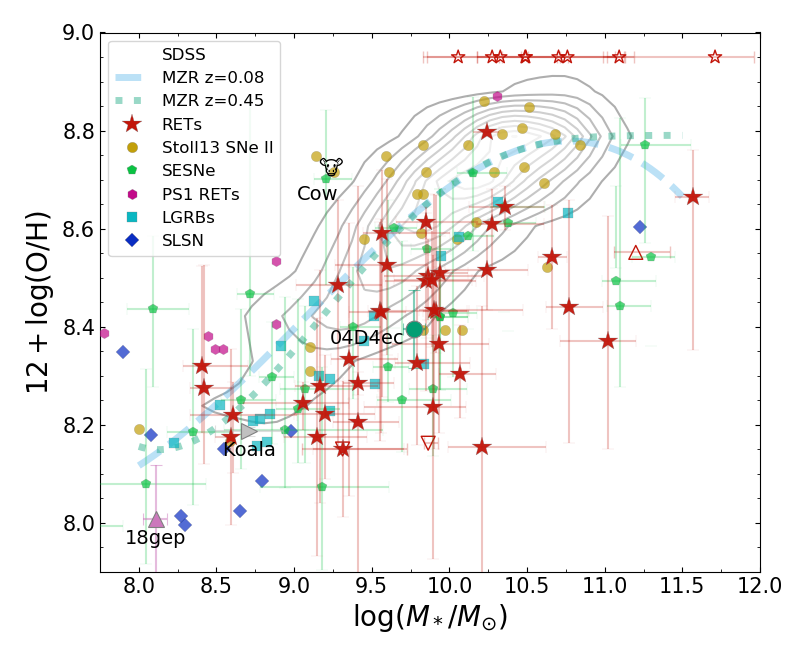
\includegraphics[width=\textwidth]{figs/RET_MZR.png}
\caption{The mass-metallicity relation (MZR) for RET host galaxies.
\label{fig:mzr}}
\end{figure*}

\begin{figure}
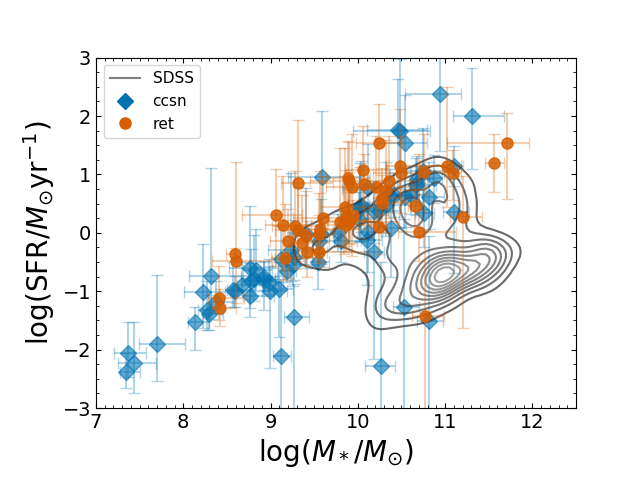
\includegraphics[width=0.5\textwidth]{figs/SFR_Mike.png}
\caption{The SFR of RET hosts, compared to CCSNe and the low-z SDSS sample.
\label{fig:sfms_sfr}}
\end{figure}

\begin{figure}
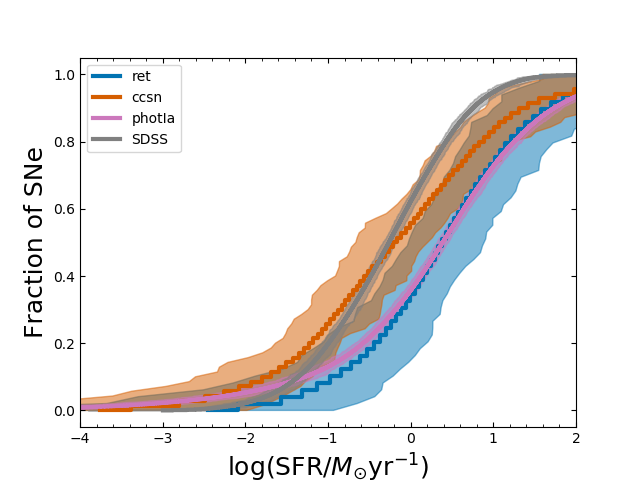
\includegraphics[width=0.5\textwidth]{figs/cum_SFR_mike.png}
\caption{Cumulative distributions of the SFR of RET hosts, compared to CCSNe and the low-z SDSS sample.
\label{fig:sfr_cum}}
\end{figure}

\begin{figure}
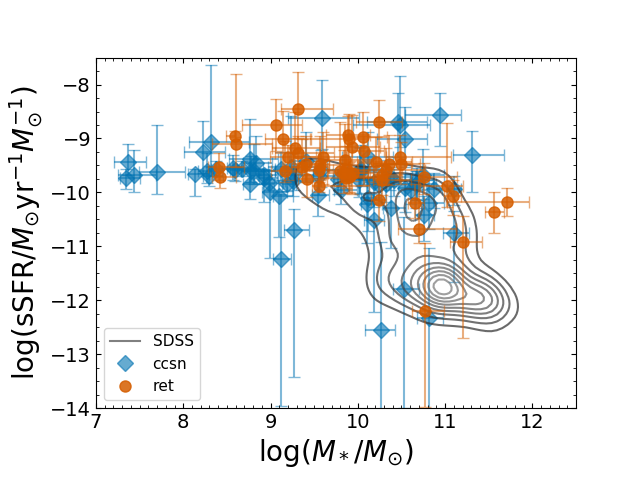
\includegraphics[width=0.5\textwidth]{figs/sSFR_Mike.png}
\caption{The sSFR of RET hosts, compared to CCSNe and the low-z SDSS sample.
\label{fig:sfms_ssfr}}
\end{figure}

\begin{figure}
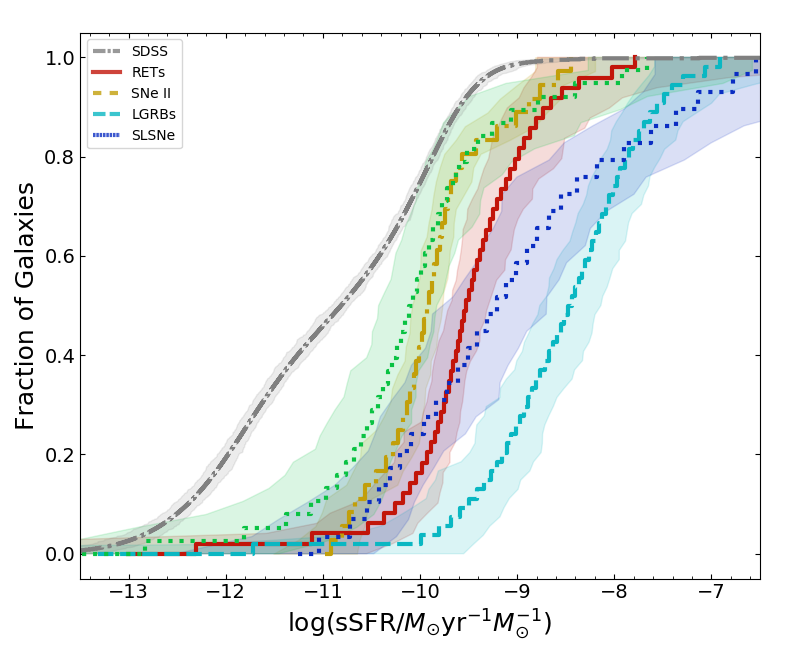
\includegraphics[width=0.5\textwidth]{figs/cum_sSFR_mike.png}
\caption{Cumulative distributions of the sSFR of RET hosts, compared to CCSNe and the low-z SDSS sample.
\label{fig:sfr_cum}}
\end{figure}


\section{Host galaxy properties}
\label{sec:analysis} % used for referring to this section from elsewhere
\subsection{Stellar Mass \label{subsec:res_mass}}

\subsection{Star formation rate \label{subsec:res_sfr}}

\subsection{Metallicity \label{subsec:res_metallicity}}

\section{Discussion \label{sec:disc}}

\subsection{Transient - host galaxy correlations}



\section{Conclusions}

The last numbered section should briefly summarise what has been done, and describe
the final conclusions which the authors draw from their work.

\section*{Acknowledgements}

The Acknowledgements section is not numbered. Here you can thank helpful
colleagues, acknowledge funding agencies, telescopes and facilities used etc.
Try to keep it short.

%%%%%%%%%%%%%%%%%%%%%%%%%%%%%%%%%%%%%%%%%%%%%%%%%%

%%%%%%%%%%%%%%%%%%%% REFERENCES %%%%%%%%%%%%%%%%%%

% The best way to enter references is to use BibTeX:

\bibliographystyle{mnras}
\bibliography{PhilMendeley} % if your bibtex file is called example.bib


% Alternatively you could enter them by hand, like this:
% This method is tedious and prone to error if you have lots of references
%\begin{thebibliography}{99}
%\bibitem[\protect\citeauthoryear{Author}{2012}]{Author2012}
%Author A.~N., 2013, Journal of Improbable Astronomy, 1, 1
%\bibitem[\protect\citeauthoryear{Others}{2013}]{Others2013}
%Others S., 2012, Journal of Interesting Stuff, 17, 198
%\end{thebibliography}

%%%%%%%%%%%%%%%%%%%%%%%%%%%%%%%%%%%%%%%%%%%%%%%%%%

%%%%%%%%%%%%%%%%% APPENDICES %%%%%%%%%%%%%%%%%%%%%

\appendix

\section{Some extra material}

If you want to present additional material which would interrupt the flow of the main paper,
it can be placed in an Appendix which appears after the list of references.

%%%%%%%%%%%%%%%%%%%%%%%%%%%%%%%%%%%%%%%%%%%%%%%%%%


% Don't change these lines
\bsp	% typesetting comment
\label{lastpage}
\end{document}

% End of mnras_template.tex